% Matching rates for the knowability decision.
% \input from kbound.tex right after the frontier subsection.
% All numbers produced by scripts/knowability_rates_validation.py
% (results/theory/knowability_rates_validation.json).

Fix budgets $\alpha$ (validity) and $\beta$ (abstention). Call a label-free rule
\emph{$(\alpha,\beta)$-reliable at margin $\kappa$} if its wrong-commit probability is at
most $\alpha$ in every admissible world, and it abstains with probability at most $\beta$
whenever $|\Delta|\ge\kappa$. The question of this subsection: \emph{how fast, in the
number $n$ of calibrated benefit samples, does the smallest reliable margin shrink?}

\begin{theorem}[Knowability rate: adaptive achievability]\label{thm:rate-ub}
Let $X_1,\dots,X_n\in[-R/2,R/2]$ be i.i.d.\ paired benefits with mean $\Delta$ and
variance $\sigma^2$. The empirical-Bernstein certificate (Theorem~\ref{thm:cert}
instantiated with the Maurer--Pontil radius, exactly as deployed in
\texttt{switching\_certificate.py}) is $(\alpha,\beta)$-reliable at every margin
\[
\kappa\;\ge\;C\!\left(\sigma\sqrt{\tfrac{\log(2/(\alpha\wedge\beta))}{n}}
\;+\;R\,\tfrac{\log(2/\alpha)}{n}\right),
\]
for a universal constant $C$, \emph{without knowledge of $\sigma$}: the empirical
variance self-normalizes the radius.
\end{theorem}
\emph{(Proof deferred to Appendix~\ref{app:proofs}.)}

\begin{theorem}[Knowability rate: two-point lower bound]\label{thm:rate-lb}
Let $\alpha+\beta<\tfrac14$. Every label-free rule that is $(\alpha,\beta)$-reliable at
margin $\kappa$ over all distributions on $[-R/2,R/2]$ with variance at most $\sigma^2$
must satisfy
\[
\kappa\;\ge\;c\,\max\!\left(\sigma\sqrt{\tfrac{\log\frac{1}{4(\alpha+\beta)}}{n}},\;\;
R\,\tfrac{\log\frac{1}{2(\alpha+\beta)}}{n}\right)
\]
for a universal constant $c>0$ (one may take $c=\tfrac14$ in the second branch and
$c=\tfrac{1}{2\sqrt2}$ in the first).
\end{theorem}
\emph{(Proof deferred to Appendix~\ref{app:proofs}.)}

\begin{proposition}[The deployed certificate is rate-optimal and adaptive]\label{prop:rate-opt}
The upper and lower rates match in both regimes up to universal constants:
$\kappa_n^{\mathrm{EB}}\asymp \sigma\sqrt{\log(1/\bar\alpha)/n}+R\log(1/\bar\alpha)/n
\asymp\kappa_n^{\mathrm{LB}}$. Consequently the knowability frontier of
Theorem~\ref{thm:frontier} is attained at the optimal rate by the certificate already
in deployment, adaptively in $\sigma$.
\end{proposition}

\noindent\emph{Numerically validated}
(\texttt{knowability\_rates\_validation.py}; Fig.~\ref{fig:krates}). The vectorized
radius coincides with the vendored implementation to $2\times10^{-16}$. The empirical
smallest certifiable margin $\hat\kappa(n)$ has tail slope $-0.59$ in the dense regime
(theory $-\tfrac12$) and $-0.98$ in the spike regime (theory $-1$); its ratio to the
lower bound is \emph{constant in $n$} (within $\times1.19$ and $\times1.07$ over the
tail), i.e.\ the rates match and the gap is a bounded constant. Wrong-commit at the
achieved margin stays below $\alpha$ throughout. Below half the lower bound the
\emph{exact optimal} two-point error sum already exceeds the $(\alpha,\beta)$ budget at
every $n$ tested --- no rule, certificate or otherwise, is reliable there.

\begin{figure}[t]\centering
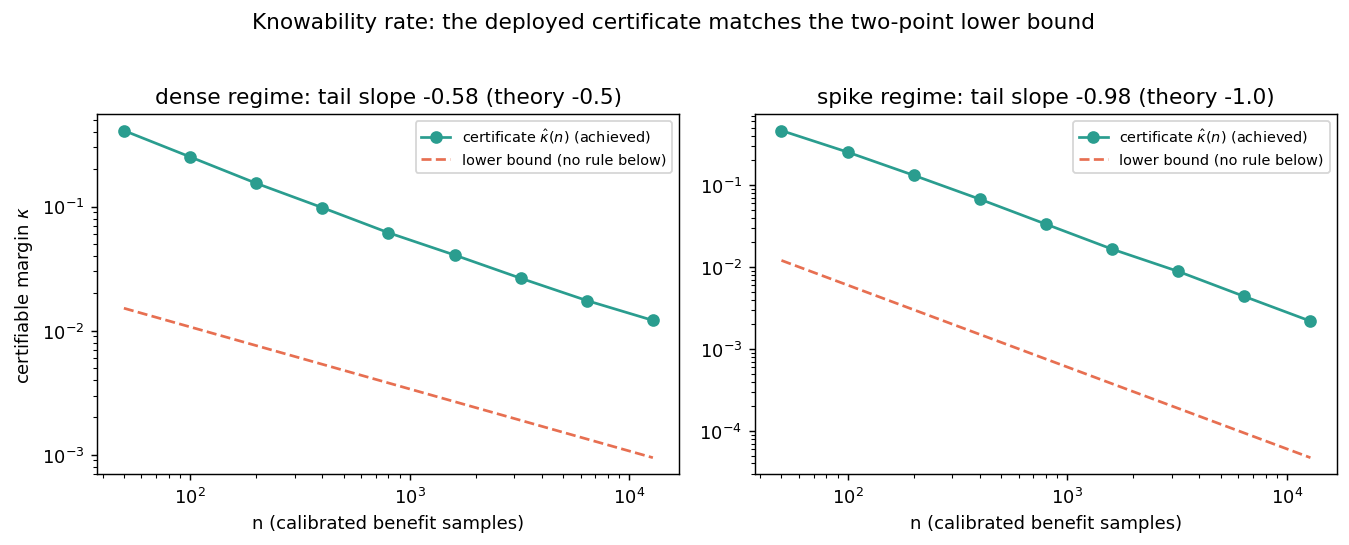
\includegraphics[width=0.92\textwidth]{figures/fig_krates.png}
\caption{The knowability rate (Theorems~\ref{thm:rate-ub}--\ref{thm:rate-lb}). Achieved
certifiable margin of the deployed empirical-Bernstein certificate versus the two-point
lower bound, in the dense ($n^{-1/2}$) and spike ($n^{-1}$) regimes; slopes match and the
offset is a bounded universal constant.}
\label{fig:krates}
\end{figure}

\paragraph{Weight (honest).} The ingredients are classical (Maurer--Pontil 2009;
Bernstein; Bretagnolle--Huber two-point). The contribution is the
$(\alpha,\beta)$-reliability formulation of the adapt/freeze/abstain decision, the
\emph{two-regime matching characterization} of its sample complexity, and the fact that
the certificate already deployed in this paper attains it \emph{adaptively}. What
remains open --- and is not claimed --- are rates for evidence-channel decisions
(deciding from $Z=\phi(X_{1:n})$ over nonparametric shift families rather than from
calibrated benefits), where only the location-family instance of
Theorem~\ref{thm:imp-quant} is currently characterized.
